\documentclass[a4paper,12pt,openright,titlepage,oneside]{book}

%\usepackage[english,brazil]{babel}
%Define regra de gramática para separar síbalas {babel}
%e altera os títulos (como chapters, sections, references) para português
\usepackage[brazil]{babel}

% Define uso de caracteres acentuados no PDF gerado
% e permite copiar corretamente o texto do PDF.
\usepackage[T1]{fontenc}
\usepackage[utf8]{inputenc}

% Adição do pacote do template da UnB
\usepackage{styles/template-FT-UnB/ft2unb}

\DeclareGraphicsExtensions{.jpg,.pdf,.mps,.png,.gif, .eps}
\graphicspath{images} %define diretório de imagens

%Arquivo com lista com hifenização correta de algumas palavras.
%Defina novas palavras no arquivo a medida que verificar que a hifenização automática
%etá errada para tais palavras.
%----------------DEFINE FORMA CORRETA DE HIFENIZAÇÃO PARA ALGUMAS PALAVRAS ----------------
\hyphenation{cons-tru-a}
\hyphenation{e-xem-plo}
\hyphenation{e-xem-plar}
\hyphenation{e-le-men-to}
\hyphenation{e-le-men-tar}
\hyphenation{ma-nu-al}
\hyphenation{res-pos-ta}
\hyphenation{ca-rac-te-ris-ti-ca}
\hyphenation{ca-rac-te-ris-ti-cas}
\hyphenation{ca-rac-te-ris-ti-co}
\hyphenation{ca-rac-te-ris-ti-cos}
\hyphenation{cor-res-pon-den-ci-as}
\hyphenation{cons-tru-am}
\hyphenation{re-a-li-za-da}
\hyphenation{re-a-li-za-do}
\hyphenation{re-a-li-za-das}
\hyphenation{re-a-li-za-dos}
\hyphenation{i-ne-xis-ten-cia}
\hyphenation{i-ne-xis-te}
\hyphenation{e-xis-te}
\hyphenation{di-fe-ren-te}
\hyphenation{di-fe-ren-tes}
\hyphenation{dei-xan-do}
\hyphenation{ins-ta-la-do} 
\hyphenation{ins-ta-la-dos} 
\hyphenation{ins-ta-la-da}
\hyphenation{ins-ta-la-das}
\hyphenation{re-gis-tra-do}
\hyphenation{re-gis-tra-dos}
\hyphenation{re-gis-tra-da}
\hyphenation{re-gis-tra-das}
\hyphenation{des-cre-ve}
\hyphenation{res-pei-to}
\hyphenation{re-a-li-za}
\hyphenation{re-a-li-zar}
\hyphenation{a-tu-a-li-zar}
\hyphenation{a-tu-a-li-zan-do}
\hyphenation{a-tu-a-li-za-do}
\hyphenation{a-tu-a-li-za-da}
\hyphenation{fun-ci-o-na-li-da-de}
\hyphenation{pos-si-bi-li-da-de}
\hyphenation{dis-po-si-ti-vo}
\hyphenation{dis-po-si-ti-vos}
\hyphenation{e-xis-te}
\hyphenation{e-xis-tir}
\hyphenation{des-co-ber-ta}
\hyphenation{des-co-ber-to}
\hyphenation{de-sig-nar}
\hyphenation{de-sig-na-do}
\hyphenation{o-pe-ra-ci-o-nais} 
\hyphenation{o-pe-ra-ci-o-nal}
\hyphenation{con-si-de-ra-do}
\hyphenation{con-si-de-ra-dos}
\hyphenation{ou-tro}
\hyphenation{ou-tra}
\hyphenation{ou-tros}
\hyphenation{ou-tras}
\hyphenation{e-xis-ten-te}
\hyphenation{e-xis-ten-tes}
\hyphenation{LuaOnTV}
\hyphenation{De-fi-ni-tion}
%------------------------------------------------------------------------------------------

% ALTERE OS VALORES DENTRO DAS CHAVES DOS COMANDOS NESTA SEÇÃO PARA INCLUIR OS SEUS DADOS E DADOS DA SUA
% DISSERTAÇÃO DE MESTRADO OU TESE DE DOUTORADO
% -----------------------------------------------------------------------------------------------------

%\onehalfspacing
\title{Previsão de insuficiência cardíaca com aprendizado de máquina voltado para aplicações}
\author{André Filipe Caldas Laranjeira}
\date{2021-05-21} %data da defesa
\coverbackgroundimg{images/capa_fundo}

\grau{Bacharel}
\area{Engenharia da computação} %Nome do curso
\departamento{Ciência da computação} %Nome do departamento
\faculdade{INSTITUTO DE CIÊNCIAS EXATAS} %Nome da faculdade/instituto
\siglafaculdade{IE} %Sigla da faculdade/instituto
\siglaarea{CIC} %Sigla do departamento
\tipodemonografia{Monografia} %Dissertação ou Tese
\programa{Bacharelado} %Mestrado ou Doutorado
\autorendereco{Área Octogonal Sul 2, Bloco G, Apartamento 601; Brasília} %Endereço do autor da dissertação/tese
\totalpgs{147} %total de páginas atualmente na sua dissertação
\dia{21} %dia da defesa
\mes{Maio} %mês da defesa
\ano{2021} %ano da defesa
\numpublicacao{xxx/AAAA} %número da publicação (após a defesa, tal número deve ser obtido na secretaria)

%PPGENE.DM  = Programa de Pós Graduação em ENgenharia Elétrica.Dissertação de Mestrado
%PPGENE.TD  = Programa de Pós Graduação em ENgenharia Elétrica.Tese de Doutorado
\siglapublicacao{?}

\titulolinhai{Previsão de insuficiência cardíaca}
\titulolinhaii{com aprendizado de máquina}
\titulolinhaiii{voltado para aplicações}
\titulolinhaiv{}

\autori{André Filipe Caldas Laranjeira}
%Caso seu nome não caiba em uma única linha, divida ele nos comandos abaixo
%\autorii{}
%\autoriii{}

\membrodabancai{Prof. Dr. Alexandre Ricardo Soares Romariz, FT/UnB}
\membrodabancaifuncao{Orientador}
\membrodabancaii{Prof. Fulano de Tal 2, ENE/UnB}
\membrodabancaiifuncao{Examinador interno}
\membrodabancaiii{Prof. Fulano de Tal 3, ENE/UnB}
\membrodabancaiiifuncao{Examinador interno}
\membrodabancaiv{Prof. Fulano de Tal 4, EESC/USP}
\membrodabancaivfuncao{Examinador externo}
\membrodabancav{}
\membrodabancavfuncao{}
% -----------------------------------------------------------------------------------------------------

%line-numbers, inputencoding=utf8/latin1
%Define o estilo para listagens de código fonte
\lstset{
  numbers=left, %numeração de linhas à esquerda
  stepnumber=1,
  firstnumber=1,
  numberstyle=\tiny,
  extendedchars=true,
  frame=none,
  basicstyle=\footnotesize,
  stringstyle=\ttfamily,
  showstringspaces=false,
  %language=Java, %deve ser definida na inclusão de cada trecho de código, pois podem existir linguagens diferentes em exemplos diferentes
  breaklines=true,
  breakautoindent=true,
  %estilos de comentário de uma e várias linhas
  morecomment=[l]{--}, morecomment=[s]{/*}{*/}, morecomment=[s]{<!--}{-->}, morecomment=[s]{--[[}{--]]}
}

% Adição de metadados no PDF (propriedades do documento PDF)
\makeatletter
	 \hypersetup{
		 pdftoolbar=true,        % show Acrobat’s toolbar?
		 pdfmenubar=true,        % show Acrobat’s menu?
		 pdffitwindow=false,     % window fit to page when opened
		 pdfstartview={FitH},    % fits the width of the page to the window
		 pdftitle={\@title},
		 pdfauthor={\@author},
		 pdfsubject={\tipodemonografianome \ de\ \programastr \ em\ \areastr},   % subject of the document
		 pdfcreationdate={\pdfdate}
	 }
\makeatother


\makeindex
\makenomenclature %Necessário para gerar lista de siglas


\begin{document}

	\pdfbookmark[0]{Agradecimentos}{agradecimentos}
	\chapter*{Agradecimentos}

Agradeço a Deus por ter me abençoado e me guiado durante todo o meu curso, cuidando de minha vida de maneira maravilhosa.
Agradeço à minha família por ter me sustentado até aqui e me proporcionado amor e encorajamento.
Agradeço aos meus professores por tudo o que eles me ensinaram e pelos desafios que eles me propuseram.
Agradeço aos meus colegas de curso por terem me ajudado ao longo do curso e me inspirado a sempre dar o melhor de mim.

	Inclua o resumo aqui.

	\pdfbookmark[0]{Sumário}{sumario}
	\sumario

	\pdfbookmark[0]{Lista de Figuras}{listafiguras}
	\listadefiguras

	\pdfbookmark[0]{Lista de Tabelas}{listatabelas}
	\listadetabelas

	\pdfbookmark[0]{Lista de Códigos Fonte}{listacodigosfonte}
	\listadecodigosfonte

	\renewcommand{\nomname}{LISTA DE TERMOS E SIGLAS} %Define um caption à lista de siglas
	%Inclui a lista de siglas
	\pdfbookmark[0]{Lista de Termos e Siglas}{nomenclatura}
	\printnomenclature[2.5cm]

	\mainmatter %Inicia a numeracao normal cardinal
	\setcounter{page}{1} \pagenumbering{arabic} \pagestyle{plain}

	\include{sections/chapters/01_introducao_teorica}
	\chapter{Introdução} \label{introducao}

% Este trabalho Lorem ipsum dolor sit amet, consectetuer adipiscing elit. Ut purus elit, vestibulum ut, placerat ac, adipiscing vitae, felis. Curabitur dictum gravida mauris. Nam arcu libero, nonummy eget, consectetuer id, vulputate a, magna. Donec vehicula augue eu neque. Pellentesque habitant morbi tristique senectus et netus et malesuada fames ac turpis egestas. Mauris ut leo. Cras viverra metus rhoncus sem. Nulla et lectus vestibulum urna fringilla ultrices. Phasellus eu tellus sit amet tortor gravida placerat. Integer sapien est, iaculis in, pretium quis, viverra ac, nunc. Praesent eget sem vel leo ultrices bibendum. Aenean faucibus. Morbi dolor nulla, malesuada eu, pulvinar at, mollis ac, nulla. Curabitur auctor semper nulla. Donec varius orci eget risus. Duis nibh mi, congue eu, accumsan eleifend, sagittis quis, diam. Duis eget orci sit amet orci dignissim rutrum.
%
% Nam dui ligula, fringilla a, euismod sodales, sollicitudin vel, wisi. Morbi auctor lorem non justo. Nam lacus libero, pretium at, lobortis vitae, ultricies et, tellus. Donec aliquet, tortor sed accumsan bibendum, erat ligula aliquet magna, vitae ornare odio metus a mi. Morbi ac orci et nisl hendrerit mollis. Suspendisse ut massa. Cras nec ante. Pellentesque a nulla. Cum sociis natoque penatibus et magnis dis parturient montes, nascetur ridiculus mus. Aliquam tincidunt urna. Nulla ullamcorper vestibulum turpis. Pellentesque cursus luctus mauris.
%
% O trabalho está organizado como segue. O capítulo  \ref{capitulo1} apresenta detalhes sobre a arquitetura proposta. O capítulo \ref{capitulo2} apresenta os protocolos de comunicação utilizados. Por fim, o capítulo \ref{conclusao} apresenta as conclusões e trabalhos futuros propostos.

	\chapter{Procedimento adotado} \label{procedimento_adotado}

Neste capítulo, o procedimento adotado ao longo do trabalho é detalhado com o intuito de permitir ao leitor compreender melhor a lógica por trás de algumas escolhas feitas no decorrer do trabalho e de explorar alguns detalhes importantes da implementação dos módulos de programação.

\section{Conjunto de dados}

Como descrito na introdução, o intuito deste trabalho foi elaborar um projeto que utilizasse aprendizado de máquinas e proporcionasse alguma utilidade prática. Para isso, foi necessária a escolha de um conjunto de dados que possibilitasse a criação de uma aplicação completa com base em aprendizado de máquinas em tempo útil para a realização deste trabalho. Tendo isso em mente, a decisão recaiu sobre um conjunto de dados\cite{larxel_dataset} originado de um artigo científico\cite{chicco2020} voltado para o estudo de aprendizado de máquinas para a previsão de ocorrência de insuficiência cardíaca.

O conjunto de dados escolhido\cite{larxel_dataset} contém 299 registros de pacientes, cada um consistindo em 11 parâmetros relacionados à saúde geral e cardíaca de um paciente, 1 parâmetro indicando o tempo de acompanhamento médico do paciente e 1 resultado indicando se o paciente veio à óbito durante o acompanhamento realizado. Dessa forma, trata-se de um conjunto de dados pequeno, de fácil compreensão, que pudesse ser explorado com um certo grau de profundidade em um curto espaço de tempo, e com uma clara utilidade prática de auxiliar a prevenção da ocorrência de insuficiência cardíaca em pacientes com base em uma previsão realizada por meio de aprendizado de máquinas.

Além das características úteis do conjunto de dados em si para a realização deste trabalho, o artigo científico que originou o conjunto de dados\cite{chicco2020} consiste em um ótimo estudo comparativo do desempenho de diferentes tipos de modelos de dados na previsão de insuficiência cardíaca com base no conjunto de dados em si, proporcionando uma referência útil para a realização de escolhas do tipo de modelo de aprendizado de máquinas a ser utilizado no conjunto de dados e para a comparação dos resultados atingidos no treinamento de modelos de aprendizado de máquinas.

Apesar dessas excelentes qualidades, devemos ressaltar que o conjunto de dados escolhido não é sem falhas. A baixa quantidade de registros no conjunto de dados faz com que o treinamento de modelos de aprendizado de máquinas seja extremamente suscetível à \textit{overfitting}, resultando em um modelo que não forneça bons resultados em aplicações práticas. Também podemos notar que a baixa quantidade de registros em que o paciente veio à óbito, agravada pelas subdivisões do conjunto de dados em dados de treinamento, de teste e de validação, pode gerar modelos com um viés para previsões positivas, aumentando a probabilidade de que o modelo de aprendizado de máquinas gere falsos negativos, em que o sistema não prediz a insuficiência cardíaca e o paciente vem à óbito. A forma como essas limitações da base de dados foram tratadas será descrita posteriormente.

\section{Modelos de treinamento}

Com a escolha do conjunto de dados feita, o próximo passo seria definir quais tipos de modelos de treinamento de aprendizagem de máquinas seriam avaliados para uso na aplicação e estabelecer um método específico de avaliação para permitir a comparação entre os diferentes modelos de treinamento e determinar qual deveria ser utilizado na aplicação.

\subsection{Tipos de modelos testados}

Inicialmente, o autor pretendia avaliar o desempenho apenas de modelos do tipo redes neuronais de perceptron multicamada por ter maior familiaridade com esse tipo de modelo. Entretanto, a leitura da análise realizada e dos resultados obtidos no artigo científico\cite{chicco2020} que originou o conjunto de dados utilizado\cite{larxel_dataset}, bem como o tempo necessário para o treinamento de um único modelo de perceptron multicamada, levaram o autor a avaliar também modelos do tipo florestas randômicas, os quais obtiveram a melhor acurácia de previsão de acordo com os resultados do artigo científico mencionado e podem ser treinados em uma fração do tempo de treinamento de modelos do tipo perceptron multicamada.

\subsection{Método de avaliação dos modelos de treinamento de aprendizado de máquinas}

Com o intuito de comparar diferentes modelos de treinamento de aprendizado de máquinas, um método padrão de avaliação foi adotado com base no método utilizado no artigo científico\cite{chicco2020} mencionado. Esta subseção, com o intuito de justificar algumas das escolhas feitas na montagem do método de avaliação adotado, descreve formalmente tanto o método de avaliação de modelos de treinamento utilizado no artigo científico, como o método de treinamento utilizado neste trabalho.

\subsubsection{Método de avaliação de modelos de treinamento utilizado no artigo científico}

O artigo científico\cite{chicco2020} em que o conjunto de dados\cite{larxel_dataset} foi primeiramente apresentado e que buscou estudar vários aspectos do aprendizado de máquinas aplicado ao conjunto de dados utilizou um método específico para avaliar quais foram os melhores modelos de aprendizado de máquinas. Esse método consistiu em dois submétodos diferentes para modelos com otimização de hiper-parâmetros e para modelos sem otimização de hiper-parâmetros.

Para tipos de modelos com otimização de hiper-parâmetros, o conjunto de dados foi dividido em 60\% de dados para treinamento, 20\% de dados para validação e 20\% de dados para teste. Primeiramente, vários modelos com diferentes hiper-parâmetros foram treinados com o subconjunto de dados de treinamento com o intuito de encontrar o conjunto de hiper-parâmetros que gerasse o melhor coeficiente de correlação de Matthews (MCC) relativo à previsão feita sobre o subconjunto de dados de validação. Esse conjunto de hiper-parâmetros então foi utilizado em um novo modelo, treinado com o subconjunto de dados de treinamento, para obter o coeficiente de correlação de Matthews (MCC) relativo à previsão feita sobre o subconjunto de dados de teste. Esse procedimento foi realizado sobre 100 diferentes partições do conjunto de dados, para que a média e mediana dos 100 resultados de coeficiente de correlação de Matthews (MCC) relativos às previsões feitas sobre os subconjuntos de dados de teste com aquele tipo de modelo fossem calculados.

Para tipos de modelos sem otimização de hiper-parâmetros, o conjunto de dados foi dividido em 80\% de dados para treinamento e 20\% de dados para teste. Um modelo foi treinado com o subconjunto de dados de treinamento para obter o coeficiente de correlação de Matthews (MCC) relativo à previsão feita sobre o subconjunto de dados de teste. Esse procedimento foi realizado sobre 100 diferentes partições do conjunto de dados, para que a média e mediana dos 100 resultados de coeficiente de correlação de Matthews (MCC) relativos às previsões feitas sobre os subconjuntos de dados de teste com aquele tipo de modelo fossem calculados.

\subsubsection{Método de avaliação de modelos de treinamento utilizado neste trabalho}

Neste trabalho, o método utilizado para avaliar quais modelos de treinamento obtiveram os melhores resultados se baseou no método de avaliação utilizado no artigo científico\cite{chicco2020}, mas com algumas alterações.

Em primeiro lugar, 100 inteiros de 32 bits sem sinal foram gerados e armazenados em um arquivo para serem utilizados como sementes na aleatoriedade inerente ao particionamento do conjunto de dados\cite{larxel_dataset}, de forma que todos os modelos agora utilizam as mesmas partições do conjunto de dados para realizarem seu treinamento e obterem seus resultados de validação e teste. Essa mudança foi feita com o intuito de permitir a replicação dos resultados obtidos e proporcionar uma forma mais justa de comparação entre diferentes modelos com diferentes hiper-parâmetros. Além disso, como o tempo de treinamento de alguns modelos pode ser consideravelmente longo, esse técnica permite que a obtenção de um resultado de validação ou teste para um mesmo modelo seja dividida em mais de uma execução, dado que um subconjunto de dados de validação e teste é fixo para uma dada semente escolhida.

Em segundo lugar, a otimização de hiper-parâmetros não pôde ser feita da mesma forma que o artigo científico, pois a quantidade de combinações de hiper-parâmetros existente não permitiria que todas as variações de hiper-parâmetros fossem testadas para um dado modelo e uma dada partição do conjunto de dados. Dessa forma, decidiu-se que a única otimização de hiper-parâmetros feita seria na quantidade de épocas de treinamento para modelos do tipo perceptron multicamada. O número de épocas escolhido para treinamento na obtenção dos resultados de teste será equivalente à época em que o modelo teve a menor perda nos dados de validação (\textit{early stopping}). Para os demais parâmetros, decidiu-se adotar o seguinte procedimento: várias variações de hiper-parâmetros seriam utilizadas para se obter o resultado de predição sobre os subconjuntos de validação do primeiro quinto das partições de dados disponíveis (20), e as combinações de hiper-parâmetros com os resultados mais promissores (mais especificamente, os modelos que estiveram entre os melhores 20\%) em relação ao subconjunto de validação seriam testadas sobre todos os subconjuntos de teste disponíveis (100) com o intuito de se calcular os seus resultados de predição. Isso permitiria que uma gigantesca quantidade de variações de hiper-parâmetros fosse experimentada para cada modelo, com apenas as variações de hiper-parâmetros mais promissoras sendo realmente testadas em todas as 100 possíveis partições do conjunto de dados disponível. Além disso, como o escopo desse trabalho envolve menos a comparação de diferentes modelos e mais a busca por um único conjunto de hiper-parâmetros que forneça bons resultados, acredito que esse formato de análise seria mais adequado que aquele utilizado no artigo científico em que diferentes combinações de hiper-parâmetros poderiam ser utilizadas em diferentes partições de dados no cálculo do resultado de teste de um modelo.

A medida utilizada para medir o desempenho de um modelo (nos resultados de validação e teste) foi a média da acurácia (accuracy) obtida em cada particionamento do conjunto de dados, em oposição ao uso do coeficiente de correlação de Matthews (MCC) utilizado no artigo científico.

Portanto, podemos resumir o procedimento adotado neste trabalho como sendo, para um dado conjunto de modelos com diferentes hiper-parâmetros, a obtenção dos resultados de validação para o primeiro quinto das sementes disponíveis e o cálculo subsequente dos resultados de teste com todas as sementes disponíveis para os modelos entre os melhores 20\% no quesito melhor média de acurácia para os dados de validação. Os resultados de validação influenciariam na escolha de quais modelos seriam utilizados para o cálculo de resultados de teste e também, no caso de modelos do tipo perceptron multicamada, na escolha do número de épocas de treinamento (\textit{early stopping}) para a obtenção de resultados de teste.

Por meio deste método de avaliação, espera-se que as falhas inerentes ao conjunto de dados utilizado sejam mitigadas. A utilização do critério de melhor média de acurácia na previsão de dados de 20 subconjuntos de validação e de 100 subconjuntos de teste é uma forma de se compensar a propensão a \textit{overfitting} e a viés no treinamento com esse conjunto de dados. Isso ocorre pois a existência de múltiplos subconjuntos distintos de treinamento assegura que os melhores modelos serão aqueles capazes de obter resultados consistentes na previsão de validação e de teste em diversos cenários, desfavorecendo combinações de hiper-parâmetros mais suscetíveis à geração de modelos que apresentem \textit{overfitting} e viés. Embora essa abordagem não solucione por completo as dificuldades apresentadas, sua utilização é um bom recurso na ausência de um conjunto de dados mais robusto e representativo da realidade.

\section{Programação da avaliação do treinamento}

Com os tipos de modelos a serem avaliados e o método de avaliação determinados, o próximo passo foi criar um programa na linguagem de programação \textit{Python} para se automatizar a aplicação do método de avaliação em diferentes modelos de treinamento e salvar os resultados obtidos. Além disso, conforme sugestão do professor orientador deste trabalho, um segundo programa foi feito com o intuito de permitir que os resultados de avaliação obtidos fossem mais facilmente visualizados em formatos gráficos.

Ambos os programas foram construídos de maneira modularizada e buscando capturar a intenção do autor ao programá-los pela utilização de nomes significativos para variáveis e funções e pela utilização de funções com um único propósito sempre que possível. Dessa forma, essa seção não tem o intuito de descrever todos os detalhes de implementação dos programas, mas sim fazer uma descrição geral da forma como os programas funcionam, apresentando ao leitor imagens e trechos de código explicativos.

\subsection{Programa para automatizar a avaliação}

O programa para automatizar a avaliação dos modelos de treinamento foi escrito no arquivo \textit{main.py} e permite que o usuário defina um conjunto de modelos de treinamento (não necessariamente do mesmo tipo de modelo) com diferentes hiperparâmetros, aplique um método de avaliação sobre os modelos definidos e salve os resultados obtidos. O usuário pode passar como argumentos na chamada do programa o tamanho do subconjunto de validação (utilizado apenas se o tipo de modelo requerer dados de validação), o tamanho do subconjunto de teste e uma \textit{flag} para que o programa cronometre o tempo decorrido durante a avaliação. Naturalmente, o tamanho do subconjunto de validação e o tamanho do subconjunto de teste têm como valor padrão 20\%, conforme especificado anteriormente no método adotado, mas o usuário tem a liberdade para alterar esses valores para utilizar o programa em outras aplicações. Também é importante ressaltar que o programa possui um argumento de ajuda para explicar o uso dos demais argumentos e um argumento de versão.

Além dessas configurações por passagem de argumentos, o corpo do programa pode ser modificado para alterar o funcionamento do programa. Pelo corpo do programa, o usuário pode definir o arquivo que contém o conjunto de dados a ser utilizado e quais colunas desse conjunto serão utilizadas como características de treinamento e rótulos, qual arquivo contém as sementes de aleatoriedade, quais modelos de treinamento serão testados nessa avaliação, o número da avaliação em si e o número de particionamentos do conjunto de dados utilizados para validação e teste. A modularização do programa permite que essas características sejam todas definidas como parâmetros de construção de classes, tornando sua modificação simples e intuitiva e reduzindo bastante o tamanho do programa principal em si.

Como exemplo simples da modularização do programa, apresentamos o trecho de código que constrói a classe de extrator de conjunto de dados utilizada para ler os dados contidos em um arquivo de conjunto de dados \ref{list:main_dataset_extractor}. Nesse trecho de código, a classe \textit{DatasetExtractor} foi importada do módulo \textit{data\_extractors.py}, o qual foi criado pelo autor para encapsular a lógica de leitura de dados de arquivos \textit{csv}. Caso o usuário queira modificar o arquivo de conjunto de dados utilizado, as colunas de características de treinamento utilizadas ou as colunas de rótulo utilizadas, basta alterar os parâmetros fornecidos ao construtor da classe.

\lstset{caption=Construção do extrator de conjunto de dados no programa de avaliação dos modelos de treinamento, label=list:main_dataset_extractor}
\begin{lstlisting}[language=python]
dataset_extractor = DatasetExtractor(
    dataset_file_name='./data/data.csv',
    feature_columns_list=[
        'age',
        'anaemia',
        'creatinine_phosphokinase',
        'diabetes',
        'ejection_fraction',
        'high_blood_pressure',
        'platelets',
        'serum_creatinine',
        'sex',
        'smoking'
    ],
    label_columns_list=['DEATH_EVENT'],
    train_size=args.train_size,
    validation_size=args.validation_size
)
\end{lstlisting}

Após o usuário definir as configurações desejadas no corpo do programa e executar o programa com os argumentos apropriados, o programa iniciará a avaliação dos modelos de treinamento definidos. O tempo médio de avaliação depende da quantidade de modelos avaliados, do tipo dos modelos avaliados e dos hiperparâmetros dos modelos em si. As avaliações realizadas pelo autor que utilizaram modelos do tipo florestas randômicas foram relativamente rápidas, demorando algumas horas para serem executadas quando centenas de modelos haviam sido definidos. Já as avaliações feitas pelo autor com modelos do tipo perceptron multicamada foram consideravelmente lentas, demorando de 36 a 48 horas para serem executadas quando apenas 5 modelos haviam sido definidos. Essa discrepância significativa foi um grande entrave para a realização de mais avaliações com modelos do tipo perceptron multicamada.

Após o programa ter sido iniciado, algumas mensagens serão mostradas na tela para informar o progresso da avaliação. Após a avaliação ter sido finalizada, os resultados obtidos serão também mostrados na tela para conhecimento do usuário e salvos em um arquivo com extensão \textit{csv}. O arquivo de resultados armazena, para cada modelo avaliado, o posicionamento do modelo em um rankeamento iniciado em 0 (porque essa posição é originada a partir de uma lista ordenada, a qual é indexada em 0), o tipo do modelo, os hiperparâmetros do modelo, as acurácias de previsão para os subconjuntos de validação dos particionamentos utilizados para validação e a média dessas acurácias, e, caso o modelo tenha sido utilizado para realizar previsões nos subconjuntos de teste, as acurácias de previsão para os subconjuntos de teste dos particionamentos utilizados para teste e a média dessas acurácias. Podemos visualizar um exemplo de arquivo de resultados aberto no \textit{LibreOffice Calc} e com algumas estilizações aplicadas na figura \ref{fig:example_evaluation_results}.

\begin{figure}[h]
	\centering
	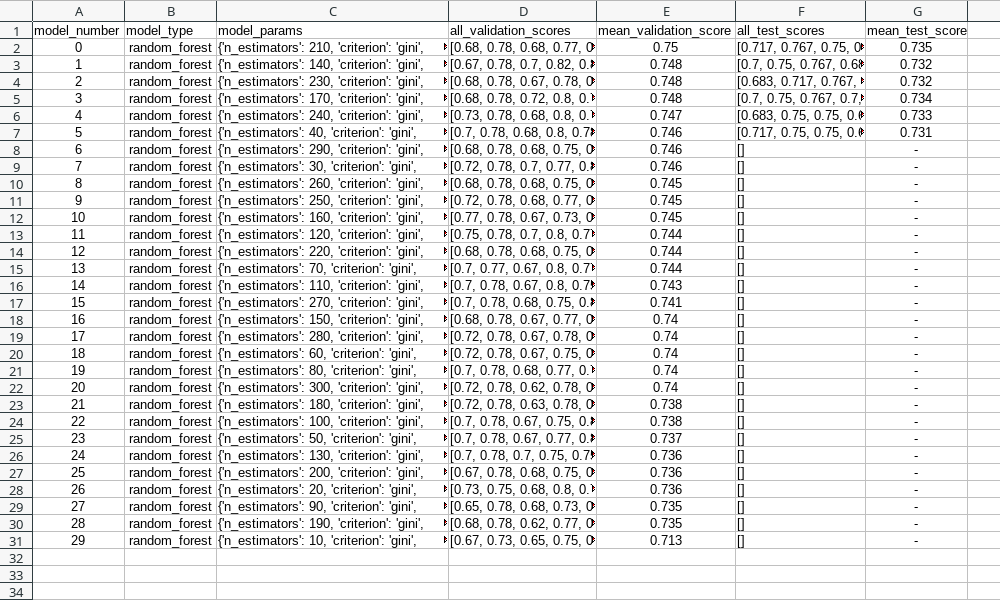
\includegraphics[scale=0.42]{images/exemplo_resultados_avaliacao.png}
	\caption{Exemplo de arquivo de resultados de avaliação aberto no programa \textit{LibreOffice Calc} e com algumas estilizações.}
	\label{fig:example_evaluation_results}
\end{figure}

Para facilitar a identificação dos resultados de avaliação, o programa tenta gravar os resultados em um arquivo na pasta \textit{results} com o nome \textit{E[Número da avaliação com 4 dígitos].csv} (e.g: \textit{results/E0001.csv}). Caso o número da avaliação não tenha sido fornecido, o programa tenta gravar os dados no arquivo \textit{results/results\_save.csv}. Caso o programa não consiga gravar os resultados em um desses arquivos por algum motivo, como, por exemplo, a inexistência da pasta \textit{results}, o programa ainda tenta realizar uma segunda gravação dos resultados, no diretório de onde o programa foi chamado, em um arquivo de \textit{fallback} de nome \textit{fallback\_results\_save.csv}.

\subsection{Programa para gerar gráficos dos resultados}

O programa para gerar gráficos de resultados foi escrito no arquivo \textit{plot\_results.py} e permite que o usuário selecione um modelo de uma das avaliações realizadas e gere uma representação gráfica dos resultados obtidos para esse modelo. O usuário pode passar como argumentos na chamada do programa o número da avaliação selecionada, o número do modelo selecionado, a ação almejada do programa (apenas mostar o gráfico gerado ou salvar o gráfico gerado em um arquivo), um nome de arquivo para receber o gráfico gerado, o tipo de gráfico a ser gerado (gráfico de barras, gráfico de caixa ou histograma) e a categoria de resultados a ser analisada (validação, teste ou uma comparação entre ambos).

O usuário é livre para combinar esses argumentos de maneira a extrair o maior valor possível dos resultados de avaliação, mas deve-se ressaltar que o argumento de nome de arquivo não será utilizado se a ação escolhida for apenas mostrar o gráfico gerado e que valores inválidos de número de avaliação ou de número de modelo geraram mensagens de erro. Também é importante notar que a execução do programa deve ser feita a partir do diretório \textit{AI}, para que o programa consiga ler adequadamente os arquivos da pasta \textit{results}. Por fim, é importante ressaltar que o programa possui um argumento de ajuda para explicar o uso dos demais argumentos e um argumento de versão.

Diferente do programa de avaliação automática de modelos de treinamento, este programa não possui configurações a serem alteradas no corpo do programa porque todas as opções de configuração são fornecidas por argumentos de chamada e repassadas para o construtor de classe utilizado e para a chamada de método realizada (a lógica do programa em si se resume a exatamente uma construção de classe e uma chamada de método devido a modularização utilizada).

Após o programa ser chamado, a classe construída utiliza um extrator de dados feito pelo autor para ler os dados do arquivo de resultados selecionado e gera, por meio da biblioteca \textit{matplotlib}, o gráfico desejado contendo os resultados lidos. Se necessário, esse gráfico então é salvo em um arquivo cujo nome é fornecido pelo usuário. Se o usuário não especificar o nome de arquivo desejado, o nome de arquivo \textit{plot\_output.png} é utilizado. Caso o programa não consiga salvar o gráfico gerado com o nome de arquivo fornecido, o programa ainda tenta realizar uma segunda gravação, no diretório de onde o programa foi chamado, em um arquivo de \textit{fallback} de nome \textit{fallback\_plot\_output.png}.

Para exemplificar o funcionamento do programa, fornecemos a imagem \ref{fig:example_results_plot}, a qual contém o gráfico de barras \ref{fig:example_results_barplot}, o gráfico de caixa \ref{fig:example_results_boxplot} e o histograma \ref{fig:example_results_histogram} gerados com os resultados de validação e de teste do melhor modelo (rankeamento 0) da avaliação número 1.

\begin{figure}[h]
	\centering
  \subfigure[Gráfico de barras]{
    \centering
    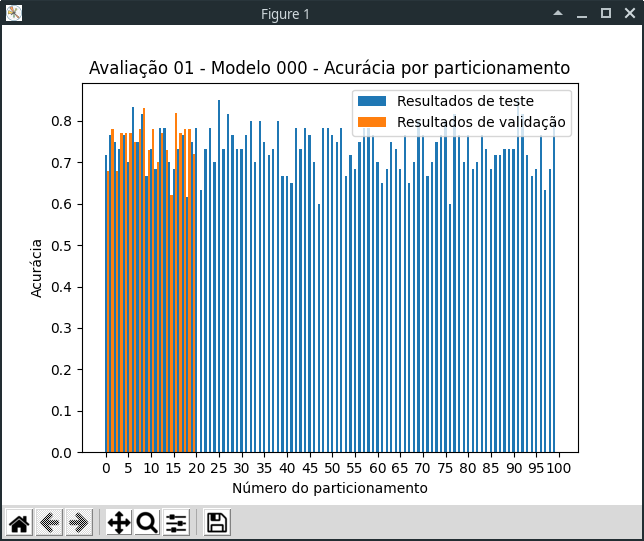
\includegraphics[scale=0.3]{images/exemplo_grafico_barras_resultados.png}
    \label{fig:example_results_barplot}
  }
  \subfigure[Gráfico de caixa]{
    \centering
    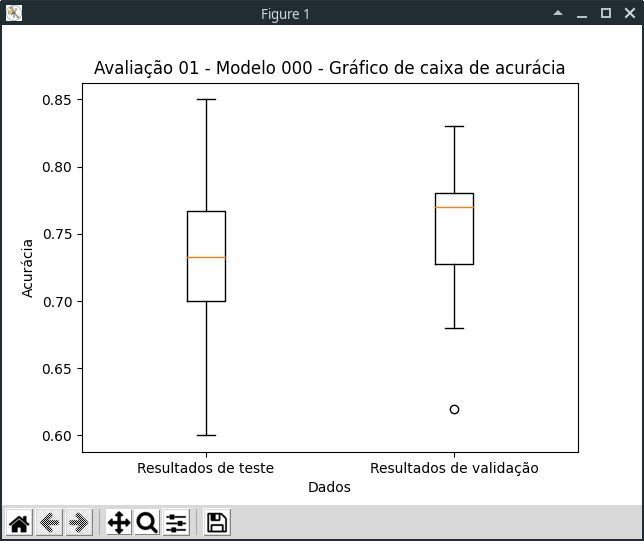
\includegraphics[scale=0.3]{images/exemplo_grafico_caixa_resultados.png}
    \label{fig:example_results_boxplot}
  }
  \subfigure[Histograma]{
    \centering
    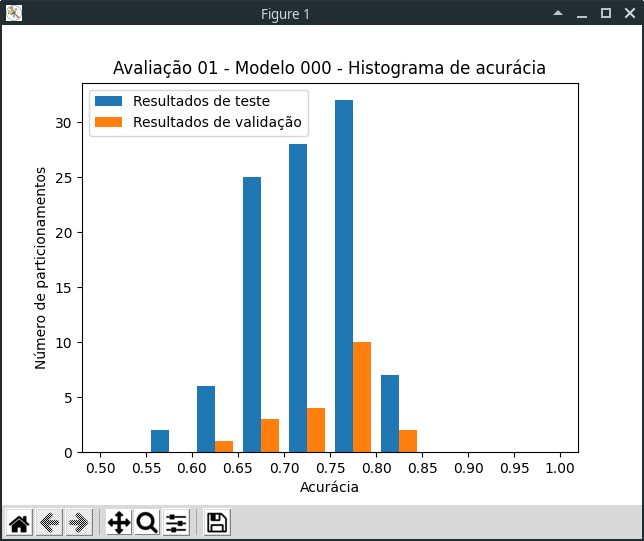
\includegraphics[scale=0.3]{images/exemplo_histograma_resultados.png}
    \label{fig:example_results_histogram}
  }
	\caption{Exemplos de gráficos de resultados gerados pela execução do programa \textit{plot\_results.py}.}
	\label{fig:example_results_plot}
\end{figure}


%label cria um rótulo para o objeto, para permitir que ele seja referenciado com o comando \ref{nome-do-rotulo}


% Neste capítulo é apresentada uma arquitetura para provimento de comércio eletrônico
% para o Sistema Brasileiro de TV Digital (SBTVD) \nomenclature{SBTVD}{Sistema Brasileiro de TV Digital}. A mesma é uma arquitetura distribuída, baseada em componentes
% reutilizáveis, os \textit{Web Services}, conhecida como Arquitetura Orientada a Serviços.
%
% Segundo \cite{soares2007ginga}:
%
% \begin{quote}
% 	Lorem ipsum dolor sit amet, consectetuer adipiscing elit. Ut purus elit, vesti- bulum ut, placerat ac, adipiscing vitae, felis. Curabitur dictum gravida mauris. Nam arcu libero, nonummy eget, consectetuer id, vulputate a, magna.
% \end{quote}
%
% Desta forma, a arquitetura proposta foi definida, incluindo a implementação de um \textit{framework} de comunicação (baseado nos protocolos HTTP e SOAP) que é apresentado sucintamente neste capítulo, e em mais detalhes no Capítulo \ref{capitulo2}. Mais detalhes podem ser consultados em \cite{soares2007ginga}. Veja um exemplo na Listagem \ref{list:server}, que foi adaptada de \url{http://manoelcampos.com}.
%
% Lorem ipsum dolor sit amet, consectetuer adipiscing elit. Ut purus elit, vestibulum ut, placerat ac, adipiscing vitae, felis. Curabitur dictum gravida mauris. Nam arcu libero, no- nummy eget, consectetuer id, vulputate a, magna. Donec vehicula augue eu neque. Pel- lentesque habitant morbi tristique senectus et netus et malesuada fames ac turpis egestas. Mauris ut leo. Cras viverra metus rhoncus sem. Nulla et lectus vestibulum urna fringilla ultrices. Phasellus eu tellus sit amet tortor gravida placerat. Integer sapien est, iaculis in, pretium quis, viverra ac, nunc. Praesent eget sem vel leo ultrices bibendum. Aenean fauci- bus. Morbi dolor nulla, malesuada eu, pulvinar at, mollis ac, nulla. Curabitur auctor semper nulla. Donec varius orci eget risus. Duis nibh mi, congue eu, accumsan eleifend, sagittis quis, diam. Duis eget orci sit amet orci dignissim rutrum.
%
% Nulla malesuada porttitor diam. Donec felis erat, congue non, volutpat at, tincidunt tristi- que, libero. Vivamus viverra fermentum felis. Donec nonummy pellentesque ante. Phasellus adipiscing semper elit. Proin fermentum massa ac quam. Sed diam turpis, molestie vitae, placerat a, molestie nec, leo. Maecenas lacinia. Nam ipsum ligula, eleifend at, accumsan nec, suscipit a, ipsum. Morbi blandit ligula feugiat magna. Nunc eleifend consequat lorem. Sed lacinia nulla vitae enim. Pellentesque tincidunt purus vel magna. Integer non enim. Praesent euismod nunc eu purus. Donec bibendum quam in tellus. Nullam cursus pulvinar lectus. Donec et mi. Nam vulputate metus eu enim. Vestibulum pellentesque felis eu massa.
%
% \lstset{caption=Exemplo de aplicação servidora, label=list:server}
% \begin{lstlisting}[language=C]
% int main()
% {
%     FILE *fp;     int len;
%     static const int SIZE = 1024;
%     struct sockaddr_in me, target;
%     int sock=socket(AF_INET,SOCK_DGRAM,0);
%     char arquivo[SIZE];
%     me.sin_family=AF_INET;
%     me.sin_addr.s_addr=htonl(INADDR_ANY); // endereco IP local
%     me.sin_port=htons(0); // porta local (0=auto assign)
%     bind(sock,(struct sockaddr *)&me,sizeof(me));
%     target.sin_family=AF_INET;
%     target.sin_addr.s_addr=inet_addr("192.168.68.217"); // host local
%     target.sin_port=htons(8450); // porta de destino
%
%     if ((fp = fopen("video1.mp4","rb")) == NULL){
%         printf("Arquivo nao pode ser aberto.\n"); return -1;
%     }
%
%     while(!feof(fp)) {
%         len = fread(arquivo, 1, sizeof(arquivo), fp);
%         sendto(sock,arquivo,sizeof(arquivo),0,(struct sockaddr *)&target,sizeof(target));
%     }
%     sendto(sock,"FIM",sizeof("FIM"),0,(struct sockaddr *)&target,sizeof(target));
%     close(sock);
%     return 0;
% }
% \end{lstlisting}

	\chapter{Resultados} \label{resultados}


% \section{Uma associação}
%
% % Gera 3 parágrafos com texto aleatório, apenas para exemplo. Apague o comando para remover tal texto.
% \lipsum[1-3]
%
%
% \subsection{Motivos para abortar uma associação}
%
% %lista não numerada
% \begin{itemize}
% 	\item primeiro item;
% 	\item segundo item;
% 	\item terceiro item;
% 	\item quarto item.
% \end{itemize}
%
% \begin{figure}[h]
% 	\centering
% 	
\includegraphics[scale=0.8]{images/red.png}
% 	\caption{Exemplo de imagem}
% 	\label{imagem1}
% \end{figure}
%
%
% Se durante o processo de configuração de uma associação for recebido como payload um hostname e esse hostname não puder ser resolvido em um tempo hábil deve se enviar um abort com a causa de erro de endereço não resolvido. Veja exemplo na Figura \ref{imagem1}.
%
%
% % Gera 4 parágrafos com texto aleatório, apenas para exemplo. Apague o comando para remover tal texto.
% \lipsum[1-4]
%
% A Tabela \ref{tabela1} a seguir apresenta os tipos de \textit{chunk} de um pacote do protocolo.
%
% \begin{table}[ht!]
%   \begin{center}
%   \setlength{\belowcaptionskip}{10pt} % espao entre caption e tabela
%   \footnotesize {
%       \begin{tabular}{|p{4cm}|p{9cm}|}
% 	  \hline
% 	  \textbf{Nome} & \textbf{Função} \\
% 	  \hline
% 	  Iniciar & Usado para iniciar uma associação \\
% 	  \hline
% 	  Confirmacao & Segunda mensagem de uma configuração de uma associação\\
% 	  \hline
% 	  Mensagem & Terceira mensagem de uma configuração de uma associação\\
% 	  \hline
% 	  Cookie & Quarta mensagem de uma configuração de uma associação\\
% 	  \hline
% 	  Dados & Dados da aplicação\\
% 	  \hline
%       \end{tabular}
%   }
%   \caption{Tipos de \textit{chunk} de um pacote SCTP}
%   \label{tabela1}
%   \end{center}
% \end{table}

	\chapter{Futuras pesquisas} \label{futuras_pesquisas}
% Como explicado no capítulo \ref{capitulo2}

	\chapter{Conclusão} \label{conclusao}

Insira sua conclusão aqui.


	%\bibliographystyle{bibliography/abnt-num} % estilo bibliográfico ABNT numérico
	%\bibliographystyle{bibliography/abnt-alf} % estilo bibliográfico ABNT alfabético
	\bibliographystyle{bibliography/sbc}  % estilo bibliográfico da Sociedade Brasileira de Computação (SBC)

	%\renewcommand{\bibname}{REFERÊNCIAS BIBLIOGRÁFICAS} %Define o Caption da seção de bibliografia
	%\addcontentsline{toc}{chapter}{REFERÊNCIAS BIBLIOGRÁFICAS}

	%não pode ter espaço entre os nomes dos arquivos bib
	\bibliography{bibliography/referencias}

	Inclua os apêndices aqui.
\end{document}
